\subsection{Problem 2.14.1}
Kursusgang 4.\\
For vectors $v=[-1,3]$ and $u=[0,4]$, find the vectors $v+u, v-u$ and $3v-2u$.
\begin{figure}[h]
    \centering
    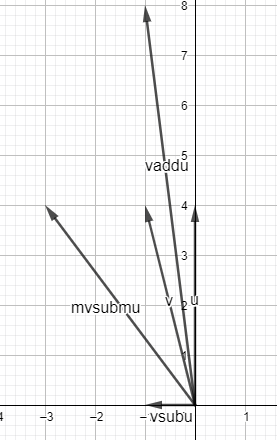
\includegraphics[]{img/vecfield2141}
    \label{ex:2141}
    \caption{Det genererede vektorfelt}
\end{figure}
De givne vektorer kan udregnes som vist i \cref{sec:addition}.
Vektorerne skal læses som $v$ add $u$ og $v$ sub $u$, hvor $m$ betyder multiplikation.